\documentclass[10pt]{article}

\usepackage[colorlinks, linkcolor=red, urlcolor=blue]{hyperref}
\usepackage{graphicx}

\usepackage{amsmath}
\usepackage{amssymb}

\title{
    {\normalsize Paper Note} \\
    {\large \href{https://openaccess.thecvf.com/content_CVPR_2020/papers/Wang_Semi-Supervised_Learning_for_Few-Shot_Image-to-Image_Translation_CVPR_2020_paper.pdf}{Semi-supervised Learning for Few-shot Image-to-Image Translation
    }} \\
    {\normalsize Project Link: \href{https://github.com/yaxingwang/SEMIT}{Github}}
}

\begin{document}
    \maketitle

    \section{Background}
        \subsection*{Previous Work}
            \begin{itemize}
                \item \href{https://arxiv.org/pdf/1806.06029.pdf}{one-shot I2I translation by first training a variational autoencoder for the seen domain and then adapting those layers related to the unseen domain.}
                \item \href{https://arxiv.org/pdf/1906.00184.pdf}{zero-shot I2I translation, employ- ing the annotated attributes of unseen categories instead of the labeled images.}
                \item \href{https://arxiv.org/pdf/1905.01723.pdf}{few-shot I2I translation in a multi-class setting. These models, however, need to be trained using large amounts of hand-annotated ground-truth labels for images of the source domain}
            \end{itemize} 

        \subsection*{Limitations}
            Labeling large-scale datasets is costly and time consuming, making those methods less applicable in practice. 
            In this paper, they overcome this limitation and explore a novel setting, few-shot I2I translation
            in which only limited labeled data is available from the source classes during training. \\
        
            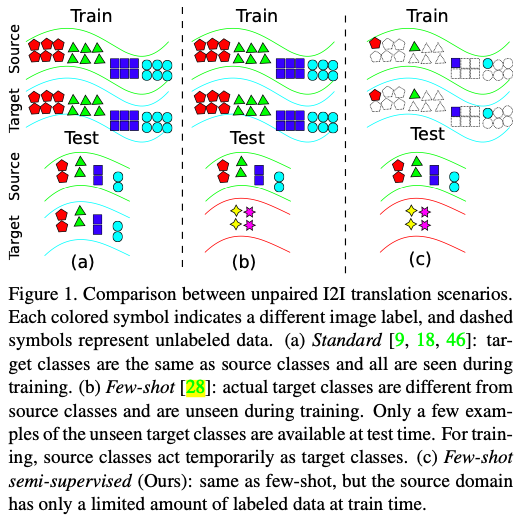
\includegraphics[width=\linewidth]{src/img/Comparison between unpaired I2I translation scenarios.png} \\ 
        
    \section*{Contribution: SEMIT}
        \subsection*{Model Overview}
            The model architecture is shown as follows: \\
            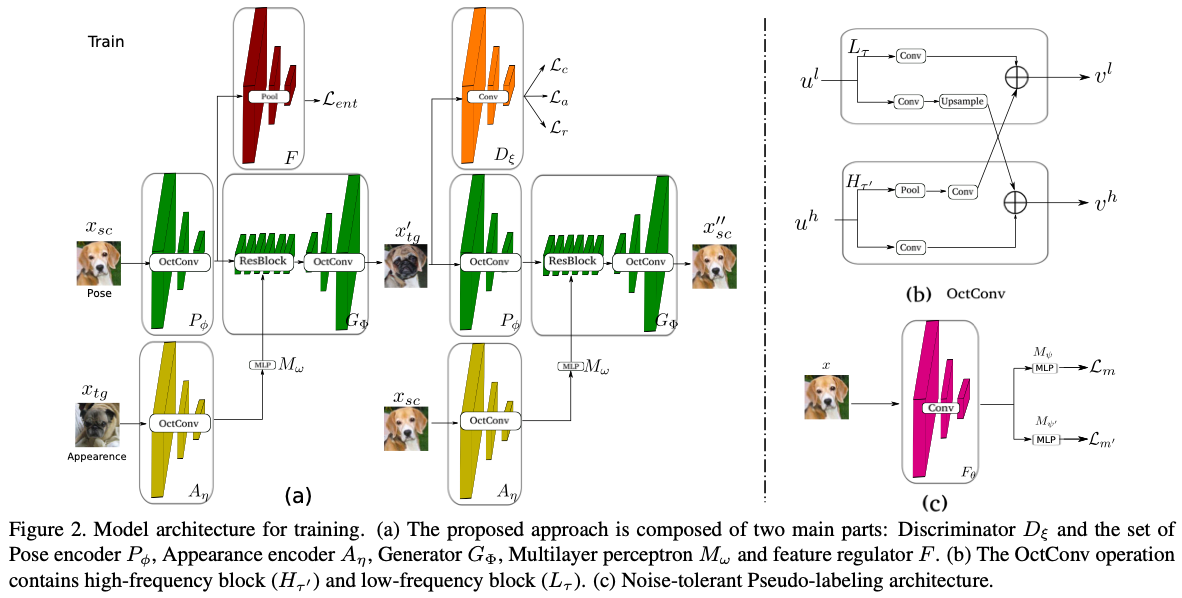
\includegraphics[width=\linewidth]{src/img/Model Architecture.png} \\
            The total loss function is: \\
            $$
                \min_{P_{\phi}, A_{\eta}, M_{\omega}, G_{\Phi}} 
                \max_{D_{\xi}} 
                \lambda_a \mathcal{L}_a + 
                \lambda_c \mathcal{L}_c + 
                \lambda_r \mathcal{L}_r + 
                \lambda_e \mathcal{L}_{ent} 
            $$
            Here, 
            \begin{equation}
                \begin{aligned}
                    & P_{\phi} \ -\  Pose\ encoder \\
                    & A_{\eta} \ -\  Appearance\ encoder \\
                    & G_{\Phi} \ -\  Generator \\
                    & M_{\omega} \ -\  Multilayer\ perceptron \\
                    & \mathcal{L}_a \ -\  Adversarial\ loss \\
                    & \mathcal{L}_c \ -\  Classfication\ loss (aux-GAN,\ to\ generate\ target-specific\ images) \\
                    & \mathcal{L}_r \ -\  Reconstruction\ loss \\
                    & \mathcal{L}_{ent} \ -\  Entropy\ regulation loss
                \end{aligned}
            \end{equation}
        
        \section*{Experiment}
            \subsection*{Datasets}
                \begin{itemize}
                    \item Animals
                    \item Birds
                    \item Flowers
                    \item Foods
                \end{itemize}
                Randomly, sample 25,000 source images from the training set and translate them to each target domain (not seen during training) \\
                1, 5, 20-shot settings for the target set. \\
            \subsection*{Evaluation}
                IS (\textit{Inception Score}) \\
                FID (\textit{Fréchet Inception Distance}) \\
                Translation Accuracy (\href{https://arxiv.org/pdf/1905.01723.pdf}{evaluate whether a model is able to generate images of the target class})
            
            \subsection*{Representative Results}
                \begin{figure}
                    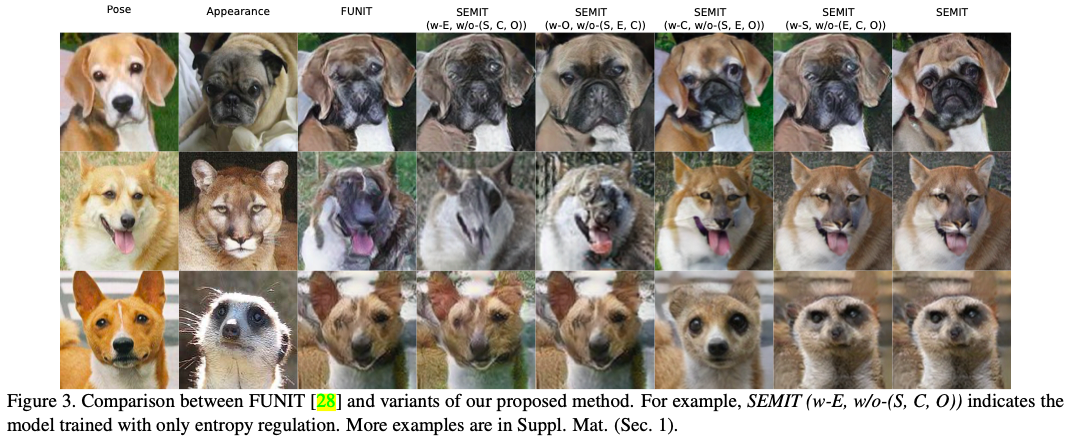
\includegraphics[width=\textwidth]{src/img/figure1.png} \\
                    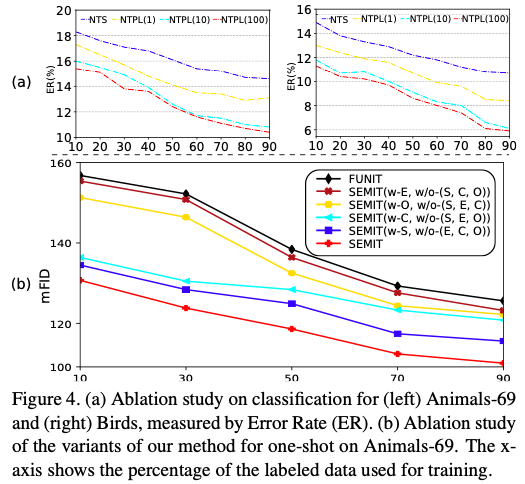
\includegraphics[width=\textwidth]{src/img/figure2.png} \\
                \end{figure}

\end{document}